\chapter{Корректность компиляции из ``обещающей'' модели в операционную модель ARMv8 POP} \label{sec:armpop}

В этой главе описывается доказательство корректности эффективной схемы компиляции из
подмножества ``обещающей'' модели памяти \cite{Kang-al:POPL17} в модель памяти ARMv8 POP \cite{Flur-al:POPL16}.
Рассмотренное подмножество ``обещающей'' модели состоит из расслабленных обращений памяти,
высвобождающего и приобретающего барьеров памяти.
Глава структурирована следующим образом.
В начале приводится высокоуровневое описание ``обещающей'' и ARMv8 POP моделей и мотивировка для доказательства
корректности компиляции между ними (раздел \ref{sec:armpop:motive}).
В разделе \ref{sec:armpop:examples} обе модели иллюстрируются на наборе примеров.
Далее приводится описание идеи доказательства корректности компиляции между ними (раздел \ref{sec:armpop:highlevel}).
В разделах \ref{sec:armpop:armmodel}  и \ref{sec:armpop:promisemodel} приводятся формальные описания моделей.
\app{TODO}
%% Разделы \ref{}
%% формальное описание 

\section{Мотивировка доказательства корректности компиляции}
\label{sec:armpop:motive}
``Обещающая'' модель (модель \Promise) --- это операционная модель памяти для языков программирования.
Она очень схожа с моделью $\OpCpp$, описанной в предыдущей главе: память представляется как множество событий,
упорядоченных метками времени, а ключевым механизмом модели также являются фронты.
Существенным отличием моделей $\Promise$ от $\OpCpp$ является то, что $\Promise$ предлагает семантический
способ для эмуляции переупорядочивания инструкций:
вместо того, чтобы откладывать операции, поток может \emph{пообещать}, что он в будущем сделает определенную запись;
обещанное сообщение становится доступным для чтения другими потоками.
Как следствие, модель $\Promise$ поддерживает больше оптимизаций и ближе к оригинальной модели C/C++11.
Негативным отличием $\Promise$ от модели $\OpCpp$ является то, что упомянутый механизм обещаний требует, чтобы
после каждого шага исполнения модели $\Promise$ происходила т.н. \emph{сертификация} --- механизм, гарантирующий
отсутствие ``значений из воздуха''. Сертификация является алгоритмически неразрешимой в случае, когда ``обещающая''
модель задана для языка, полного по Тьюрингу, и, как следствие, в этом случае для ``обещающей'' невозможно
разработать интерпретатор.
Несмотря на это, научное сообщество рассматривает ``обещающую'' модель как замену для модель памяти языков C/C++ и Java.
%% поэтому формальные результаты о модели имеют существенное значение.
Для того, чтобы модель действительно смогла стать частью стандартов этих языков, должна быть доказана корректность
компиляции во все основные целевые платформы: x86, Power, ARM.

Модель памяти ARMv8 POP является операционной моделью памяти, которая впервые описала многопоточное поведение процессорной
архитектуры ARMv8.0.
В этой версии архитектуры появилось несколько новых инструкций, которые призваны не только упростить
компиляцию из языков C/C++11, но и повысить производительность целевых программ.
Так, в частности, в модели появились отдельные инструкции приобретающего чтения и высвобождающей записи.
Кроме того, модель ARMv8 POP представляет особый интерес, т.к. она является очень слабой моделью и позволяет слабые сценарии
поведения, которые не наблюдаются в рамках других моделей памяти процессорных архитектур, таких как x86 и Power.

Для ``обещающей'' модели памяти была доказана корректность компиляции в модели x86-TSO \cite{Sewell-al:CACM10} и
Power \cite{Alglave-al:TOPLAS14} в \cite{Kang-al:POPL17}. Доказательство было основано на том, что модели x86-TSO и Power
представимы в виде набора локальных переупорядочиваний, для которых доказана корректность в ``обещающей'' модели памяти, над
более строгими моделями. Для более строгих моделей верно, что всех их сценарии поведения могут быть воспроизведены
в подмножестве ``обещающей'' модели, в котором не используется механизмы обещаний и, как следствие, сертификации.

Тот же подход не применим для модели ARMv8 POP. Так, следующая программа имеет слабый сценарий поведения с результатом $a = 1$
в модели ARMv8 POP:
%, и этот результат не может быть объяснён без обещаний:
\begin{equation*}
\tag{ARM-weak}
\begin{tabular}{c}
  $\writeInst{x}{0}; \writeInst{y}{0};$ \\
\begin{tabular}{L || L || L}
  \readInst{a}{x}; \; \valuecom{1} & \readInst{b}{x}; & \readInst{c}{y}; \\
  \writeInst{x}{1}                 & \writeInst{y}{b} & \writeInst{x}{c} \\
\end{tabular}
\end{tabular}
\end{equation*}
В этой программе любое переупорядочивание инструкций невозможно, и, как следствие, упомянутый сценарий поведения воспроизводим
в ``обещающей'' модели только с помощью механизма обещаний.

%% Приведенное в этой главе доказательство является единственным существенным формальным результатом о модели ARMv8 POP на данный момент.

\section{Модели на примерах}
\label{sec:armpop:examples}

Мы начнём обсуждение ARMv8 POP и ``обещающей'' моделей с того, что покажем как слабое поведение программы ${\rm MP}$
воспроизводится в них.
\begin{equation*}
\tag{MP}
\begin{tabular}{c}
  $\writeInst{x}{0}; \writeInst{y}{0};$ \\
\begin{tabular}{L || L}
  \writeInst{x}{1}; & \readInst{a}{y}; ~\valuecom{1} \\
  \writeInst{y}{1} & \readInst{b}{x}~ ~\valuecom{0} \\
\end{tabular}
\end{tabular}
\end{equation*}
Схема компиляции, рассмотренная в доказательстве, имеет следующий вид:
\[
  \begin{array}{c@{~~}@{~~}l@{~~}|@{~~}l@{~~}|@{~~}l@{~~}|@{~~}l}
    \textbf{Promise:} & \writeInstParam{\rlx}{x}{a} & \readInstParam{\rlx}{a}{x} &  \acqFence & \relFence \\[2pt]
    \textbf{ARMv8 POP:}     & \writeInst{x}{a}    & \readInst{a}{x}  &  \dmbLD & \dmbSY \\
  \end{array}
\]
Так как схема компиляции является биекцией на инструкциях обоих моделей, то все программы в этой главе будут представлены
в одном синтаксисе --- синтаксисе модели ARMv8 POP.

\subsection{Модель ARMv8 POP}
Модель ARMv8 POP задана операционно, и, соответственно, существует некоторая абстрактная машина, \emph{ARM машина},
которая описывает сценарии поведения в модели.
ARM машина состоит из двух компонент: \emph{подсистемы управления} (thread subsystem) и \emph{подсистемы памяти} (storage subsystem).
До некоторой степени об этих системах можно думать как о наборе вычислительных ядер (подсистема управления), которые,
выполняя программу, посылают запросы в оперативную и кэш-память (подсистема памяти).
Сама подсистема памяти в ARM машине представлена как иерархическая система \emph{буферов}, где каждый буфер является изменяемым
списком запросов. Сами запросы бывают трёх видов: на чтение, на запись и барьер памяти.

\begin{figure}

\begin{subfigure}{.33\textwidth}
  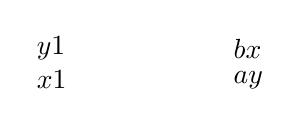
\begin{tikzpicture}[scale = 1, transform shape]
    \storageTwoThreads
    \node[right] at (1, -0.2) {\storageFont $\writeInst{x}{1}$};
    \node[right] at (1,  0.2) {\storageFont $\writeInst{y}{1}$};
    \node[right] at (3.5, -0.2) {\storageFont $\readInst{a}{y}$};
    \node[right] at (3.5,  0.2) {\storageFont $\readInst{b}{x}$};
  \end{tikzpicture}
  \caption{}
  \label{fig:armvpop:mpstorage:1}
\end{subfigure}%
\begin{subfigure}{.33\textwidth}
  \begin{tikzpicture}[scale = 1, transform shape]
    \storageTwoThreads
    \node[right] at (1,  0) {\storageFont $\writeInst{x}{1}$};
    \node[right] at (2.25, -1.6) {\storageFont $\writeInst{y}{1}$};
    \node[right] at (2.25, -1.2) {\storageFont $\readInst{a}{y}$};
    \node[right] at (2.25, -0.8) {\storageFont $\readInst{b}{x}$};
  \end{tikzpicture}
  \caption{}
  \label{fig:armvpop:mpstorage:2}
\end{subfigure}%
\begin{subfigure}{.33\textwidth}
  \begin{tikzpicture}[scale = 1, transform shape]
    \storageTwoThreads
    \node[right] at (1,  0) {\storageFont $\writeInst{x}{1}$};
    \node[right] at (2.25, -1.4) {\storageFont $\writeInst{y}{1}$};
    \node[right] at (2.25, -1) {\storageFont $\readInst{b}{x}$};
  \end{tikzpicture}
  \caption{}
  \label{fig:armvpop:mpstorage:3}
\end{subfigure}
\caption{Состояние подсистемы памяти ARMv8 POP при исполнении программы ${\rm MP}$}
\label{fig:armvpop:mpstorage}
\end{figure}

Результат $[a = 1, b = 0]$ в ARM машине может быть получен двумя способами.
Во-первых, подсистема управления имеет право исполнять инструкции не по порядку (out-of-order execution).
Так, первый поток в программе ${\rm MP}$ может отправить запрос на запись $\writeInst{y}{1}$ в подсистему памяти до запроса $\writeInst{x}{1}$,
соответственно второй поток может увидеть эти запросы в отличном от программного порядке.
Во-вторых, подсистема памяти также может переупорядочить запросы внутри себя.
Так, сначала оба потока отправляют по два запроса в подсистему памяти (см. рис. \ref{fig:armvpop:mpstorage:1}).
После подсистема переупорядочивает независимые запросы $\writeInst{x}{1}$ и $\writeInst{y}{1}$, отправляет $\writeInst{y}{1}$
в общий для двух потоков буфер, как и запросы второго потока (см. рис. \ref{fig:armvpop:mpstorage:2}).
Поскольку в общем буфере запросы $\writeInst{y}{1}$ и $\readInst{a}{y}$ находятся рядом, то подсистема памяти может послать
ответ $[a = 1]$ на запрос $\readInst{a}{y}$ в подсистему управления (cм. рис. \ref{fig:armvpop:mpstorage:3}).
После чего 

\section{Идея и структура доказательства корректности компиляции}
\label{sec:armpop:highlevel}

\section{Формальное определение модели ARMv8 POP}
\label{sec:armpop:armmodel}

\section{Формальное определение ``обещающей'' модели}
\label{sec:armpop:promisemodel}

%% В этом разделе мы формально описываем подмножество обещающей модели памяти \cite{Kang-al:POPL17}.

%% \newcommand{\figfull}{
\begin{figure*}[t]
\small
\begin{mathpar}
\vspace*{-1mm}
%
%% \inferrule[\textsc{(memory: new)}]{
%% \ %o \sqsupseteq \ra \implies \forall m' \in \lprom.\; m'.\lloc \neq m.\lloc 
%% }{\tup{\lprom, \mem}  \astep{m} \tup{\lprom, \mem \insertadd m}}
%% \and
%% \inferrule[\textsc{(memory: fulfill)}]{
%% %% \hookleftarrow \in \setofz{\insertsplit, \insertupdate} \\
%% \lprom'= \lprom \hookleftarrow m\\ \mem'= \mem \hookleftarrow m 
%% }{\tup{\lprom, \mem}  \astep{m} \tup{\lprom' \setminus \setofz{m}, \mem'}}
%% %
%% \\\vspace*{-1mm}
%
\inferrule[\textsc{(read-helper)}]{
\viewCur(\loc) \leq t
  \\\\
\viewCur'  = \viewCur \sqcup [\loc@\tau] \\
\viewAcq'   =  \viewAcq \sqcup \viewCur'
}
{{\tup{\viewCur,\viewAcq,\viewRel}}  \astep{\rlab{}{\loc}{\tau,\mrel}}
 {\tup{\viewCur',\viewAcq',\viewRel}}}
\and
\inferrule[\textsc{(write-helper)}]{
\viewCur(\loc) < t \\
\mrel = \viewRel \sqcup [\loc@\tau] \\\\
\viewCur'  = \viewCur \sqcup [\loc@\tau] \\
\viewAcq'   =  \viewAcq \sqcup \viewCur'
}
%{\tup{\tup{\viewCur,\viewAcq,\viewRel},\gsco}  \astep{\wlab:o,x,t,\mrel_\lr,\mrel_\lw} \tup{\tup{\viewCur',\viewAcq',\viewRel'},\gsco}}
{{\tup{\viewCur,\viewAcq,\viewRel}}  \astep{\wlab{}{\loc}{\tau,\mrel}} {\tup{\viewCur',\viewAcq',\viewRel}}}
%
\\\vspace*{-1mm}
%
\inferrule[\textsc{(read)}]{
  \msg{\loc}{\val}{\tau}{\mrel}\in\mem\\\\
\sigma \astep{\rlab{}{\loc}{\val}} \sigma' \\
%\tup{\tcom,\gsco} {\astep{\rlab:o,x,t,\mrel}}  \tup{\tcom',\gsco} 
{\tcom} {\astep{\rlab{}{\loc}{\tau,\mrel}}}  {\tcom'} 
}{\tup{\tup{\sigma, \tcom, \lprom}, \mem} \promTStepgen{}
  \tup{\tup{\sigma', \tcom', \lprom}, \mem}}
\and
\inferrule[\textsc{(write)}]{
\sigma \astep{\wlab{}{\loc}{\val}} \sigma' \\
{\tcom} {\astep{\wlab{}{\loc}{\tau, \mrel}}} {\tcom'} \\
m=\msg{\loc}{\val}{\tau}{\mrel}\\\\
\forall \val', \R'. \; \msg{\loc}{\val'}{\tau}{\R'} \nin M\\\\
\mem' = \mem \cup \{m\} \\ \lprom' = \lprom \setminus \{m\}
%% \tup{\lprom, \mem}  \astep{m} \tup{\lprom', \mem'} \\
}{\tup{\tup{\sigma, \tcom, \lprom}, \mem} \promTStepgen{}
  \tup{\tup{\sigma', \tcom', \lprom'}, \mem'}}
%
\\\vspace*{-1mm}
%
\inferrule[\textsc{(acq-fence)}]{
\sigma \astep{\flab{\acqo}} \sigma'
}{\tup{\tup{\sigma, \tup{\viewCur,\viewAcq,\viewRel}, \lprom}, \mem} \promTStepgen{} \\\\
  \quad \tup{\tup{\sigma', \tup{\viewAcq,\viewAcq,\viewRel}, \lprom}, \mem}}
\and
\inferrule[\textsc{(rel-fence)}]{
\sigma \astep{\flab{\relo}} \sigma'
}{\tup{\tup{\sigma, \tup{\viewCur,\viewAcq,\viewRel}, \emptyset}, \mem} \promTStepgen{} \\\\
  \quad \tup{\tup{\sigma', \tup{\viewCur,\viewAcq,\viewCur}, \emptyset}, \mem}
}
%
\\\vspace*{-1mm}
%
\inferrule[\textsc{(silent)}]{
  \\\\
  \\\\
\sigma \astep{\epsilon} \sigma'
}{\tup{\tup{\sigma, \tcom, \lprom}, \mem}  \promTStepgen{}
  \tup{\tup{\sigma', \tcom, \lprom}, \mem}}
\and
\inferrule[\textsc{(promise)}]{
  \forall \val, \R. \; \msg{m.\loc}{\val}{m.\tau}{\R} \nin M\\\\
 \lprom'= \lprom \cup \{m\}\\
 \mem'= \mem \cup \{m\} \\\\
 \forall \loc. \; \exists \val, \R. \; \msg{\loc}{\val}{m.\lmrel(\loc)}{\R} \in \mem'
 %% m.\lmrel \tmin \mem'
}{\tup{\tup{\sigma, \tcom, \lprom},\mem} \promTStepgen{}
  \tup{\tup{\sigma, \tcom, \lprom'},\mem'}}
%
\\\vspace*{-1mm}
%
\inferrule[\textsc{(global)}]{
     \angled{\TS, \Mprom} \promTStepgen{}
     \angled{\TS', \Mprom'}
%% \\\\
%%      \angled{\TS', \Mprom'} \promTStepgen{}^{*}
%%      \angled{\TS'', \Mprom''} 
%% \\\\
%% \TS''.\PromSet = \emptyset
}{
\tup{\TSf[\tId \mapsto \TS], \Mprom} \promStepgen{}
\tup{\TSf[\tId \mapsto \TS'], \Mprom'}
}
\end{mathpar}
%% \caption{Локальные переходы потоков обещающей семантики.}
\caption{Переходы обещающей машины.}
\label{fig:full-opsem-a}
\end{figure*}
%% В этом разделе мы введем обещающую модель \cite{Kang-al:POPL17} формально.

Состояние обещающей машины $\StateProm$ является парой $\angled{\TSf, M}$.
При этом $M\subset \promMessageSet$ --- это память машины, являющаяся множеством сообщений
вида  $\writeEvt{\loc}{\stval}{\tau}{\R} : \promMessageSet$, состоящих из
целевой локации, $\loc : \Loc$, значения, $\stval : \Stval$, метки времени, $\tau : \Timestamp = \mathbb{Q}$,
и фронта сообщения, $\R : \View = \Loc \rightarrow \Timestamp$.
$\TSf : \Tid \rightarrow {\sf TS}$ --- это функция, которая по идентификатору потока возвращает его состояние.
Состояние потока, $\TS : {\sf TS}$, является тройкой $\angled{\pstate, \V, \PromSet}$.
$\pstate$ --- локальное состояние потока в рамках описанной ниже помеченной системы переходов (labeled transition system, LTS).
$\V = \angled{\Rcur,\Racq,\Rrel} : \View \times \View \times \View$ --- базовый, приобретающий и высвобождающий
фронты потока. $\PromSet \subset \promMessageSet$ --- множество сообщений, которые были обещаны потоком, но еще
не выполнены.

Как было отмечено выше, обещающая модель памяти задана на помеченной системе переходов, а не на программах непосредственно. 
В приложении \ref{sec:appendixProg} приводятся синтаксис исходного языка программ и метод построения системы переходов по программе.
Сами метки в системе переходов могут быть:
(i) операцией чтения из локации $\loc$ значения $\val$ ($\rlab{}{\loc}{\val}$),
(ii) операцией записи в локацию $\loc$ значения $\val$ ($\wlab{}{\loc}{\val}$),
(iii) барьером памяти с модификатором $\FtypeProm$ ($\flab{\FtypeProm}$) или
(iv) внутреннему переходу ($\epsilon$). Последний тип описывает действия потока, которые не затрагивают память, например,
присваивание в локальную переменную и исполнение оператора условного перехода.

Перед исполнением любой программы память обещающей машины состоит из записей во все локации,
$\Mprom^{\rm init} \triangleq \{ \writeEvt{\loc}{0}{\tstamp{0}}{\R^{\rm init}} \mid \loc \in \Loc \}$,
где $\R^{\rm init} \triangleq \lambda \loc. \; \tstamp{0}$. В целом, изначальное состояние машины выглядит следующим образом:
\[
  \pinit \triangleq \angled{
     \lambda \tId. \; \angled{\pstate = \pstate^{\rm init},
                              \V = \angled{\R^{\rm init}, \R^{\rm init}, \R^{\rm init}}, \PromSet = \emptyset},
     \Mprom^{\rm init}}.
\]

Перейдем к описанию шагов исполнения в обещающей машине (см. рис. \ref{fig:full-opsem-a}).
Единственным правилом, оперирующим на всем состоянии машины, является правило $(\textsc{global})$.
В версии обещающей машины без сертификации \cite{Kang-al:POPL17} оно не несет смысловой нагрузки,
а только позволяет записать остальные правила локально для потоков (см. описание ниже).
\app{Описать сертификацию, поменять правило соответствующим образом.}

%% Основное правило перехода обещающей машины является глобальным, т.е. заданным над состоянием всей машины целиком:
%% \[
%% \frac{\begin{array}{l}
%%      \angled{\TS, \Mprom} \promTStepgen{}
%%      \angled{\TS', \Mprom'}
%% \\
%%      \angled{\TS', \Mprom'} \promTStepgen{}^{*}
%%      \angled{\TS'', \Mprom''} 
%% \end{array}
%% \qquad     \TS''.\PromSet = \emptyset
%% }{
%% \angled{\TSf[\tId \mapsto \TS], \Mprom} \promStepgen{}
%% \angled{\TSf[\tId \mapsto \TS'], \Mprom'}
%% }
%% \]
%% Данный переход требует от потока,
%% который совершает локальный переход, провести \emph{сертификацию} обещаний, т.е. показать,
%% что существует изолированный запуск потока, в рамках которого поток выполнит все свои обещания.
%начинающийся с текущим состоянием памяти машины,
\begin{description}
  \item[Выполнение приобретающего барьера] $\textsc{(acq-fence)}$
    делает базовый фронт потока $\Rcur$, равным приобретающему фронту потока $\Racq$,
    где приобретающий фронт --- объединение фронтов сообщений, прочитанных потоком к этому моменту, и меток времени записей,
    произведенных потоком.

  \item[Выполнение высвобождающего барьера] $\textsc{(rel-fence)}$
    делает высвобождающий фронт потока $\Rrel$, равным базовому фронту потока $\Rcur$.
    Как результат, фронты сообщений, которые поток добавит в память после выполнения высвобождающего барьера, будут содержать
    информацию о записях, произведенных потоком до выполнения высвобождающего барьера.%
    Кроме того, переход, соответствующий высвобождающему барьеру, имеет дополнительное ограничение --- в момент его выполнения
    у потока не должно быть невыполненных обещаний, т.е. $\PromSet$ должен быть равен пустому множеству.
  
  \item[Чтение из локации] $\loc$ $\textsc{(read)}$ поток выполняет следующим образом. Поток выбирает некоторое сообщение
    $\writeEvt{\loc}{\stval}{\tau}{\R}$ из памяти машины. При этом метка времени записи $\tau$ должна
    быть больше, чем значение базового фронта потока $\Rcur(\loc)$ а само сообщение не должно быть
    среди обещанных, но не выполненых потоком сообщений $\PromSet$.
    Это правило увеличивает базовый фронт потока на $[\loc@\tau]$, а приобретающий --- на $\R$.
    
  \item[Обещание записи] $\writeEvt{\loc}{\stval}{\tau}{\R}$ $\textsc{(promise)}$ добавляет сообщение в память машины и
    в множество $\PromSet$. При этом целевая локация $\loc$ и значение $\stval$ могут быть
    произвольными, т.е. они не зависят от локального состояния потока $\pstate$.
    Метка времени должна быть уникальной среди сообщений локации $\loc$, уже находящихся в памяти.
%%     The message view equals to a composition of the release view, $\Rrel$, and a
%%     singleton view $[\loc@\tau]$.\footnote{This is more restrictive than in the original
%%       presentation \cite{Kang-al:POPL17}, which allows to promise a write with an arbitrary message
%%       view.}
    Этот переход не обновляет фронты потока. Также легко заметить, что этот переход существенно
    недетерминирован, однако он ограничен сертификацией.
    
  \item[Выполнение обещания] $\writeEvt{\loc}{\stval}{\tau}{\R}$ $\textsc{(fulfill)}$ удаляет сообщение из множества
    невыполненных обещаний $\PromSet$. При этом данный переход должен быть возможен в
    рамках помеченной системы переходов локальных состояний, т.е. должно существовать
    состояние $\pstate'$, такое что $\pstate \xrightarrow{\wlab{}{\loc}{\stval}} \pstate'$.
    При этом метка времени $\tau$ должна быть больше значения базового фронта $\Rcur(\loc)$,
    и фронт сообщения $\R$ должен быть равен композиции высвобождающего фронта $\Rrel$
    и $[\loc@\tau]$. Переход также увеличивает базовый и приобретающий фронты потока на $[\loc@\tau]$.

  \item[Внутренний переход] $\textsc{(silent)}$ соответствует шагу исполнения потока, который не взаимодействует
    с памятью --- присваивание в локальную переменную, исполнение условного перехода или пустой операции.
    Меняет только локальное состояние потока.
\end{description}

%% \section{``Обещающая'' модель памяти} \label{sec:promise}

%% \subsection{Обещающая модель на примерах}
%% \label{sec:promiseEx}
%% В этом разделе мы приведем неформальное описание обещающей модели памяти \cite{Kang-al:POPL17} на нескольких примерах.

%% \subsubsection{Базовые элементы обещающей модели}
%% Рассмотрим программу ${\rm MP}$ (передача сообщения, message passing):
%% \begin{equation*}
%% \tag{MP}\label{ex:MP}
%% \begin{tabular}{L || L}
%%   \writeInst{x}{1}; & \readInst{a}{y}; ~\valuecom{1} \\
%%   \writeInst{y}{1}; & \readInst{b}{x}; ~\valuecom{0} \\
%% \end{tabular}
%% \end{equation*}
%% Эта программа является упрощенным вариантом шаблона, используемого для передачи
%% данных между потоками. Первый поток записывает данные в локацию $x$ и потом выставляет флаг (локация $y$),
%% что данные подготовлены; в свою очередь второй поток проверяет флаг, а потом читает данные.
%% Модель последовательной консистентности гарантирует, что если второй поток увидел, что
%% флаг выставлен ($a = 1$), то он увидит и подготовленные данные ($b = 1$).
%% Данное заключение неверно для многих слабых моделей, в том числе для обещающей и ARMv8.3
%% моделей. Рассмотрим, как слабое поведение $a = 1, b = 0$ достигается при исполнении ${\rm MP}$
%% в обещающей модели памяти.

%% %% Здесь с помощью $a$ и $b$ мы обозначаем локальные переменные потоков (регистры),
%% %% а с помощью $x$ и $y$ --- локации (адреса) в памяти, которые доступны всем потокам
%% %% в программе.
%% %% Мы используем пометки у чтений из памяти (например, $\valuecom{1}$) для того, чтобы
%% %% обозначить результат чтения в некотором интересующем нас поведении программы.

%% Обещающая модель памяти задана операционным способом. Это означает, что существует
%% некоторая абстрактная машина, связанная с моделью, которая исполняет программы
%% по шагам, и множество всех конечных состояний этой машины для некоторой программы является
%% семантикой программы в рамках данной модели. Далее мы будем использовать термин
%% \emph{обещающая машина} для обозначения упомянутой абстрактной машины.

%% Состояние обещающей машины включается в себя множество сообщений, которое называется 
%% \emph{памятью}. Мы считаем, что память перед исполнением программы содержит по сообщению
%% со значением 0 для каждой локации.
%% Так, для приведенной выше программы начальная память будет состоять из двух сообщений:
%% \[
%% M_{\rm init} = \{\angled{x:0@\tstamp{0}}, \angled{y:0@\tstamp{0}}\}
%% \]
%% Сообщение --- это тройка из локации, значения и \emph{метки времени} (timestamp,
%% в приведенном примере --- $\tstamp{0}$). Метки времени используются для упорядочивания
%% сообщений, которые связаны с одной и той же локацией.

%% Теперь покажем некоторое исполнение ${\rm MP}$, которое приводит к $a = 1, b = 0$.
%% Сначала левый поток программы ${\rm MP}$ выполняет обе записи, после чего
%% память обещающей машины содержит четыре сообщения:
%% \[
%% M = \{\angled{x:0@\tstamp{0}}, \angled{y:0@\tstamp{0}}, \angled{x:1@\tstamp{5}}, \angled{y:1@\tstamp{3.5}}\}
%% \]
%% Заметим, что метки времени новых сообщений должны быть больше, чем метки инициализирующих
%% сообщений, но между собой они никак не связаны и могли бы совпасть --- выбор меток времени
%% в обещающей машине недетерминирован. Так, конкретное значение метки времени сообщения не
%% имеет значения, важно лишь соотношение между метками сообщений, относящихся к той же локации.

%% Следующим шагом в выбранном запуске, приводящем к $a = 1, b = 0$, правый поток выполняет чтение из локации $y$.
%% Обещающая машина разрешает потоку произвести чтение из любого сообщения локации $y$ в памяти,
%% $\angled{y:0@\tstamp{0}}$ или $\angled{y:1@\tstamp{3.5}}$. Поскольку мы хотим
%% получить $a = 1$, правый поток производит чтение из сообщения с меткой времени $\tstamp{3.5}$.
%% Далее, если бы поток еще раз читал из локации $y$, ему было бы запрещено производить
%% чтение из сообщений с меткой времени меньше $\tstamp{3.5}$.
%% Интуитивно, если поток увидел более новое значение, то он больше не должен видеть более старое значение.

%% Для того, чтобы обеспечить данное свойство, у каждого потока обещающей машины есть
%% \emph{фронт} --- взгляд (view, viewfront) на память. Это функция, которая по локации возвращает
%% метку времени последнего сообщения, относящегося к этой локации, которое было увидено потоком.
%% Так, перед тем как левый поток выполнил инструкции записи, фронты левого и правого потоков
%% указывают на изначальные сообщения:
%% \[
%% T1.\Rcur = [x@\tstamp{0}, y@\tstamp{0}] \quad T2.\Rcur = [x@\tstamp{0}, y@\tstamp{0}]
%% \]
%% После того, как левый поток выполнил обе инструкции записи, он больше не может видеть
%% более старые значения. Это гарантируется тем, что его фронт по каждой локации увеличился:
%% \[
%% T1.\Rcur = [x@\tstamp{5}, y@\tstamp{3.5}] \quad T2.\Rcur = [x@\tstamp{0}, y@\tstamp{0}]
%% \]
%% После того, как правый поток выполнил чтение из сообщения $y$ с меткой времени $\tstamp{3.5}$,
%% его фронт увеличивается по $y$:
%% \[
%% T1.\Rcur = [x@\tstamp{5}, y@\tstamp{3.5}] \quad T2.\Rcur = [x@\tstamp{0}, y@\tstamp{3.5}]
%% \]
%% В программе остается невыполненной только второе чтение из локации $x$ в правом потоке.
%% Это чтение правый поток может совершить из сообщения с меткой времени $\tstamp{0}$, т.к. $T2.\Rcur(x) \le \tstamp{0}$.

%% \subsubsection{Барьеры памяти}
%% Как же гарантировать передачу сообщения между потоками в программе ${\rm MP}$, а именно запретить результат
%% $a = 1, b = 0$? Для этого нужно добавить в программу ${\rm MP}$ несколько \emph{барьеров памяти} (memory fences) ---
%% специальных инструкций, которые в реальных системах запрещают некоторые оптимизации со стороны компилятора и
%% процессора. Например, \emph{высвобождающий} (release, $\rel$) барьер используется для того, чтобы
%% запретить переупорядочивание инструкций записи со стороны компилятора,
%% а \emph{приобретающий} (acquire, $\acq$) --- инструкций чтения.
%% Так, версия программы ${\rm MP}$ с высвобождающим и приобретающим барьерами в левом и правом потоках
%% соответственно не может завершиться с результатом $a = 1, b = 0$:
%% \begin{equation*}
%% \tag{MP-rel-acq}\label{ex:MP-rel-acq}
%% \begin{tabular}{L || L}
%%   \writeInst{x}{1}; & \readInst{a}{y}; ~\valuecom{1} \\
%%   \fenceInst{\rel}; & \fenceInst{\acq}; \\
%%   \writeInst{y}{1}; & \readInst{b}{x}; ~\valuefail{0} \\
%% \end{tabular}
%% \end{equation*}

%% %% Мы показали исполнение ${\rm MP}$ в обещающей машине с результатом $a = 1, b = 0$, которое не может
%% %% быть получено попеременным исполнением команд на одном процессоре, т.е. в рамках модели последовательной
%% %% консистентности \cite{Lamport:TC79}. Если данное поведение является нежелательным, то его можно запретить
%% %% с помощью барьеров памяти (memory fences) --- специальных инструкций, которые гарантируют сохранение
%% %% которые для данной программы гарантируют
%% %% последовательную консистентность всех исполнений.
%% %% \app{TODO}
%% %% , которые в момент выполнения меняют фронты потоков и, тем самым, ограничивают
%% %% поведение потоков.

%% Для поддержки барьеров памяти нужно внести некоторые изменения в память обещающей машины ---
%% у каждого сообщения появляется свой фронт. Интуитивно, фронт сообщения $msg$ указывает на те
%% сообщения в памяти, которые становятся видны потоку, который читает из сообщения $msg$ и,
%% после этого, выполняет приобретающий барьер.

%% Так, после выполнения инструкций записи левым потоком, память машины выглядит следующим образом:
%% \[\begin{array}{l@{~}l}
%%   M = & \{\angled{x:0@\tstamp{0}, [x@\tstamp{0}]}, \angled{y:0@\tstamp{0}, [y@\tstamp{0}]}, \\
%%       & \quad
%%         \begin{array}{l@{~}l@{~}l}
%%           \angled{x:1@\tstamp{5},   & [x@\tstamp{5}, y@\tstamp{0}  &]}, \\
%%           \angled{y:1@\tstamp{3.5}, & [x@\tstamp{5}, y@\tstamp{3.5}&]}\}
%%         \end{array}
%% \end{array}\]
%% В данном случае интерес представляет фронт второго сообщения локации $y$ --- $[x@\tstamp{5}, y@\tstamp{3.5}]$.
%% После того, как левый поток выполнит чтение из этого сообщения и исполнит приобретающий барьер,
%% его фронт будет равен $[x@\tstamp{5}, y@\tstamp{3.5}]$, что запретит ему чтение из сообщения
%% $\angled{x:0@\tstamp{0}, [x@\tstamp{0}]}$.

%% Для поддержки барьеров нам также нужно добавить по два дополнительных фронта потокам --- высвобождающий и приобретающий.
%% Рассмотрим тот же запуск программы ${\rm MP}$.
%% Перед исполнением программы все три фронта левого потока равны $[x@\tstamp{0}, y@\tstamp{0}]$. После выполнения
%% инструкции записи в локацию $x$, базовый и приобретающий фронты левого потока соответственным образом растут, тогда как
%% высвобождающий остается без изменений:
%% \[T1.\Rcur[x@\tstamp{5}, y@\tstamp{0}] \quad T1.\Racq[x@\tstamp{5}, y@\tstamp{0}] \quad T1.\Rrel[x@\tstamp{0}, y@\tstamp{0}]\]
%% После выполнения барьера высвобождающий фронт становится равным базовому:
%% \[T1.\Rcur[x@\tstamp{5}, y@\tstamp{0}] \quad T1.\Racq[x@\tstamp{5}, y@\tstamp{0}] \quad T1.\Rrel[x@\tstamp{5}, y@\tstamp{0}]\]
%% Теперь, когда левый поток добавляет новое сообщение локации $y$ в память, фронт этого сообщения равен высвобождающему
%% фронту потока, увеличенному на $[y@\tstamp{3.5}]$ --- метку времени самого сообщения.

%% Перейдем к правому потоку. Его фронты также изначально равны $[x@\tstamp{0}, y@\tstamp{0}]$. После того, как поток
%% читает из сообщения $\angled{y:1@\tstamp{3.5}, [x@\tstamp{5}, y@\tstamp{3.5}]}$, его базовый фронт увеличивается на
%% метку времени самого сообщения, $[y@\tstamp{3.5}]$, тогда как приобретающий --- на фронт сообщения:
%% \[T2.\Rcur[x@\tstamp{0}, y@\tstamp{3.5}] \quad T2.\Racq[x@\tstamp{5}, y@\tstamp{3.5}] \quad T2.\Rrel[x@\tstamp{0}, y@\tstamp{0}]\]
%% Выполнение барьера приравнивает базовый фронт к приобретающему:
%% \[T2.\Rcur[x@\tstamp{5}, y@\tstamp{3.5}] \quad T2.\Racq[x@\tstamp{5}, y@\tstamp{3.5}] \quad T2.\Rrel[x@\tstamp{0}, y@\tstamp{0}]\]
%% После этого правый поток не может прочитать сообщение $\angled{x:0@\tstamp{0}, [x@\tstamp{0}]}$, т.к. $T2.\Rcur(x) > \tstamp{0}$.

%% \subsubsection{Механизм обещаний}
%% Как мы только что убедились, обещающая модель позволяет задавать поведения многопоточной программы, выходящие за
%% пределы простого попеременного исполнения потоков над обычной памятью. Это достигается за счет устройства 
%% памяти обещающей машины, которая может хранить более одного сообщения для каждой локации.
%% Тем не менее этого недостаточно для выражения всех поведений, наблюдаемых на современных архитектурах.
%% Например, следующая программа ${\rm LB}$ (load buffering) может завершиться с результатом $a = b = 1$:
%% \begin{equation*}
%% \tag{LB}\label{ex:LB}
%% \begin{tabular}{L || L}
%%   \readInst{a}{x}; ~\valuecom{1} & \readInst{b}{y}; ~\valuecom{1} \\
%%   \writeInst{y}{1}; & \writeInst{x}{1}; \\
%% \end{tabular}
%% \end{equation*}
%% Такое поведение не может наблюдаться в версии обещающей машины, описанной выше, т.к.
%% для получения $a = b = 1$ первой инструкцией должна выполниться одна из инструкций записи.
%% Архитектурные модели памяти, такие как ARMv8 POP \cite{Flur-al:POPL16}, явным образом разрешают исполнение инструкций
%% не по порядку (out of order execution). В обещающей модели нет такой возможности.
%% Зато любой поток в любой момент исполнения программы может \emph{пообещать}
%% сделать запись некоторого сообщения в память в будущем.
%% Например, первым шагом обещающей модели для программы ${\rm LB}$ может быть обещание левым потоком
%% сделать запись в локацию $y$. После этого в памяти машины появляется соответствующее сообщение:
%% \[
%% M = \{\angled{x:0@\tstamp{0}, [x@\tstamp{0}]}, \angled{y:0@\tstamp{0}, [y@\tstamp{0}]},
%%       \angled{y:1@\tstamp{2}, [x@\tstamp{0}, y@\tstamp{2}]}\}
%% \]
%% Теперь правый поток может выполнить свои инструкции --- сначала прочитать из нового сообщения,
%% а потом выполнить инструкцию записи обычным способом, без обещаний. После этого память будет содержать четыре сообщения:
%% \[
%% M = \{\angled{x:0@\tstamp{0}, [x@\tstamp{0}]}, \angled{y:0@\tstamp{0}, [y@\tstamp{0}]},
%%       \angled{y:1@\tstamp{2}, [x@\tstamp{0}, y@\tstamp{2}]}, \angled{x:1@\tstamp{2}, [x@\tstamp{2}, y@\tstamp{0}]}\},
%% \]
%% и левый поток может прочитать из сообщения $\angled{x:1@\tstamp{2}}$ и после этого выполнить обещание записать
%% сообщение $\angled{y:1@\tstamp{2}, [y@\tstamp{2}]}$ в память.

%% Как чтение из памяти потоком ограничено его базовым фронтом, так и для обещаний существует ограничение ---
%% поток не может читать из сообщений, которые он пообещал, но еще не выполнил. Для поддержания этого инварианта
%% у каждого потока имеется компонента состояния, которая хранит множество еще не выполненых обещаний.
